
\chapter{Implementacja}

\label{chap:implementation}Projekt systemu zakładał napisanie go
w języku C\# w środowisku .NET Framework 4.5~\cite{Microsoft.NET}
i umożliwienie wykonywania kodu użytkownika z bibliotek skompilowanych
do kodu zarządzalnego dla .NET Framework w wersji nie nowszej niż
4.5. Testy wykonania kodu użytkownika zostały przeprowadzone z użyciem
aplikacji napisanych w językach C\# oraz F\#. 

System Bluepath działa na klastrze węzłów obliczeniowych. Na każdym
węźle musi zostać uruchomiona binarnie zgodna wersja aplikacji (w
stopniu umożliwiającym wykonanie dowolnej metody z dowolnej klasy
będącej częścią procesu za pomocą zserializowanego uchwytu otrzymanego
w ramach zlecenia pod pewnymi warunkami opisanymi w punkcie \ref{sec:implementation-Rozproszony-watek}).
W ramach jednego z wątków uruchamiana jest usługa nasłuchująca wywołań
-- zleceń, zapytań przychodzących od pozostałych węzłów.


\section{Komunikacja}

W sieci komunikacyjnej w warstwie transportowej działa protokół TCP
\cite{rfc675,rfc793,rfc1122}, który realizuje gwarancje niezawodnego
dostarczenia wiadomości z użyciem mechanizmu potwierdzeń i retransmisji
zgodnie z założeniem przyjętym w punkcie \ref{sub:concept-Komunikacja}
ppkt. 1. Komunikacja między węzłami została zrealizowana w modelu
RPC (pkt. \ref{def:background-RPC}) za pomocą WCF (pkt. \ref{def:background-WCF}).
Połączenia realizowane są za pomocą protokołu HTTP \cite{rfc2616},
a wiadomości są przesyłane zgodnie z protokołem SOAP~\cite{W3C-SOAP11,W3C-SOAP12-part0,W3C-SOAP12-part1},
co spełnia wymagania postawione w punkcie \ref{sub:concept-Komunikacja}
ppkt. 2. Z~uwagi na losowy wybór numerów portów założono, że na maszynach
nie działa zapora ogniowa (pkt. \ref{def:background-Firewall}) blokująca
połączenia przychodzące na portach o wysokich numerach. W sieci nie
może także działać mechanizm NAT, co uniemożliwiłoby realizację bezpośredniej
komunikacji między węzłami. 

Wątek nasłuchujący jest reprezentowany przez obiekt klasy \dcscode{BluepathListener}.
Wewnętrznie tworzy on instancję klasy faktycznie nasłuchującej na
losowym porcie na wiadomości zgodne z interfejsem \dcscode{IRemoteExecutorService},
który został przedstawiony na listingu \ref{lis:implementation-Interfejs-IRemoteExecutorService},
a szczegółowy opis protokołu znajduje się w punkcie \ref{sec:implementation-Wykonawca}
poświęconym \dcsname{wykonawcom}. Dokonywana jest też rejestracja
w \dcsname{usłudze odnajdywania węzłów}. Jeżeli w ramach jednego
procesu zostanie utworzone kilka instancji klasy \dcscode{BluepathListener}
każda z nich będzie nasłuchiwała na innym porcie i posiadała własną
kolekcję \dcsname{lokalnych wykonawców}. Lista znanych \dcsname{zdalnych wykonawców}
jest współdzielona w ramach procesu przez wszystkie wątki nasłuchujące. 

W systemie każdy węzeł może komunikować się z dowolnym innym, o ile
zna jego adres IP i numer portu, pod którym działa usługa. Komunikaty,
zarówno wywołania (ang.~\dcsemph{request}) jak i wywołania zwrotne
(ang.~\dcsemph{callback}), mają charakter asynchroniczny. Istnieje
również możliwość wyłączenia wywołań zwrotnych i przełączenia systemu
w tryb pracy z odpytywaniem (ang.~\dcsemph{polling}). Wprowadza
on dodatkowe opóźnienia, co dyskwalifikuje go w przypadku prowadzenia
w klastrze faktycznych obliczeń, znajduje jednak zastosowanie w niektórych
scenariuszach realizowanych w~środowisku testowym.

\inputencoding{latin2}\begin{lstlisting}[caption={Interfejs IRemoteExecutorService},label={lis:implementation-Interfejs-IRemoteExecutorService},language={[Sharp]C},numbers=left]
[ServiceContract]
public interface IRemoteExecutorService
{
    [OperationContract]
    Guid Initialize(byte[] methodHandle);

    [OperationContract]
    void Execute(Guid eId, object[] parameters, ServiceUri callbackUri);

    [OperationContract]
    void ExecuteCallback(Guid eid, RemoteExecutorServiceResult executeResult);

    [OperationContract]
    RemoteExecutorServiceResult TryJoin(Guid eId);

    [OperationContract]
    PerformanceStatistics GetPerformanceStatistics();
}
\end{lstlisting}
\inputencoding{utf8}


\section{Usługa odnajdywania węzłów}

Obecna implementacja zawiera usługę odnajdywania węzłów zrealizowaną
w sposób scentralizowany, a każdy z węzłów podłączających się do klastra
musi znać adres IP i numer portu, pod którym działa \dcsname{usługa odnajdywania węzłów}.
Usługa udostępnia metody służące do zarejestrowania się węzła (\dcscode{Register}),
wyrejestrowania się węzła (\dcscode{Unregister}), pobrania listy
zarejestrowanych w klastrze węzłów (\dcscode{GetAvailableServices}),
oraz pobrania statystyk wydajności wszystkich węzłów w klastrze (\dcscode{GetPerformanceStatistics}).

\inputencoding{latin2}\begin{lstlisting}[caption={Interfejs ICentralizedDiscoveryService},language={[Sharp]C},numbers=left]
[ServiceContract]
public interface ICentralizedDiscoveryService
{
    [OperationContract]
    ServiceUri[] GetAvailableServices();

    [OperationContract]
    void Register(ServiceUri uri);

    [OperationContract]
    void Unregister(ServiceUri uri);

    [OperationContract]
    Task<Dictionary<ServiceUri, PerformanceStatistics>> GetPerformanceStatistics();
}
\end{lstlisting}
\inputencoding{utf8}


\section{Wątek rozproszony}

\label{sec:implementation-Rozproszony-watek}\dcscode{DistributedThread}
to klasa, której instancje reprezentują jednostkę przetwarzania w
systemie czyli \dcsname{wątek rozproszony} (patrz \ref{def:background-Rozproszony-watek}).
Wątek taki tworzony jest na podstawie delegatu \dcscode{Func} opakowującego
statyczną (nazwaną lub anonimową) metodę. Liczba parametrów wejściowych
takiej metody to maksymalnie 16 (jest to ograniczenie wprowadzone
przez deklaracje typu \dcscode{Func} dostępne w .NET Framework).
Wszystkie typy parametrów oraz typ zwracany muszą być oznaczone atrybutem
\dcscode{Serializable}. Przykład tworzenia i uruchamiania przez użytkownika
\dcsname{wątku rozproszonego} z użyciem domyślnego \dcsname{zarządcy połączeń}
i \dcsname{planisty} został przedstawiony na listingu \ref{lis:implementation-Tworzenie-i-uruchamianie-watku}.

Środowisko zakłada izolację pomiędzy wątkami: \dcsname{wątki rozproszone}
działające w~ramach jednego procesu-hosta nie mogą komunikować się
ze sobą poprzez pamięć operacyjną, a parametry, z którymi wywoływana
jest metoda są kopiowane do nowych instancji klas i struktur. Wyjątkiem
jest tutaj dostarczana przez środowisko \dcsname{pamięć rozproszona}.
W tym przypadku użytkownik powinien stosować dostarczone wraz z nią
mechanizmy synchronizacji. 

\begin{minipage}[t]{1\textwidth}%
\inputencoding{latin2}\begin{lstlisting}[caption={Tworzenie
i uruchamianie rozproszonego w�tku},label={lis:implementation-Tworzenie-i-uruchamianie-watku},language={[Sharp]C},numbers=left]
var thread = DistributedThread.Create(
    new Func<..., IBluepathCommunicationFramework, ...>((..., bluepath) => { 
        ...
        return ...; 
    }
)); 

thread.Start(...);
\end{lstlisting}
\inputencoding{utf8}%
\end{minipage}


\section{Wykonawca}

\label{sec:implementation-Wykonawca}Poniżej opisane zostały szczegóły
protokołu komunikacyjnego (rys. \ref{fig:implementation-Protokol-IRemoteExecutorService})
używanego przez węzły obliczeniowe oraz szczegóły implementacji \dcsname{wykonawców}.

\begin{figure}
\centering{}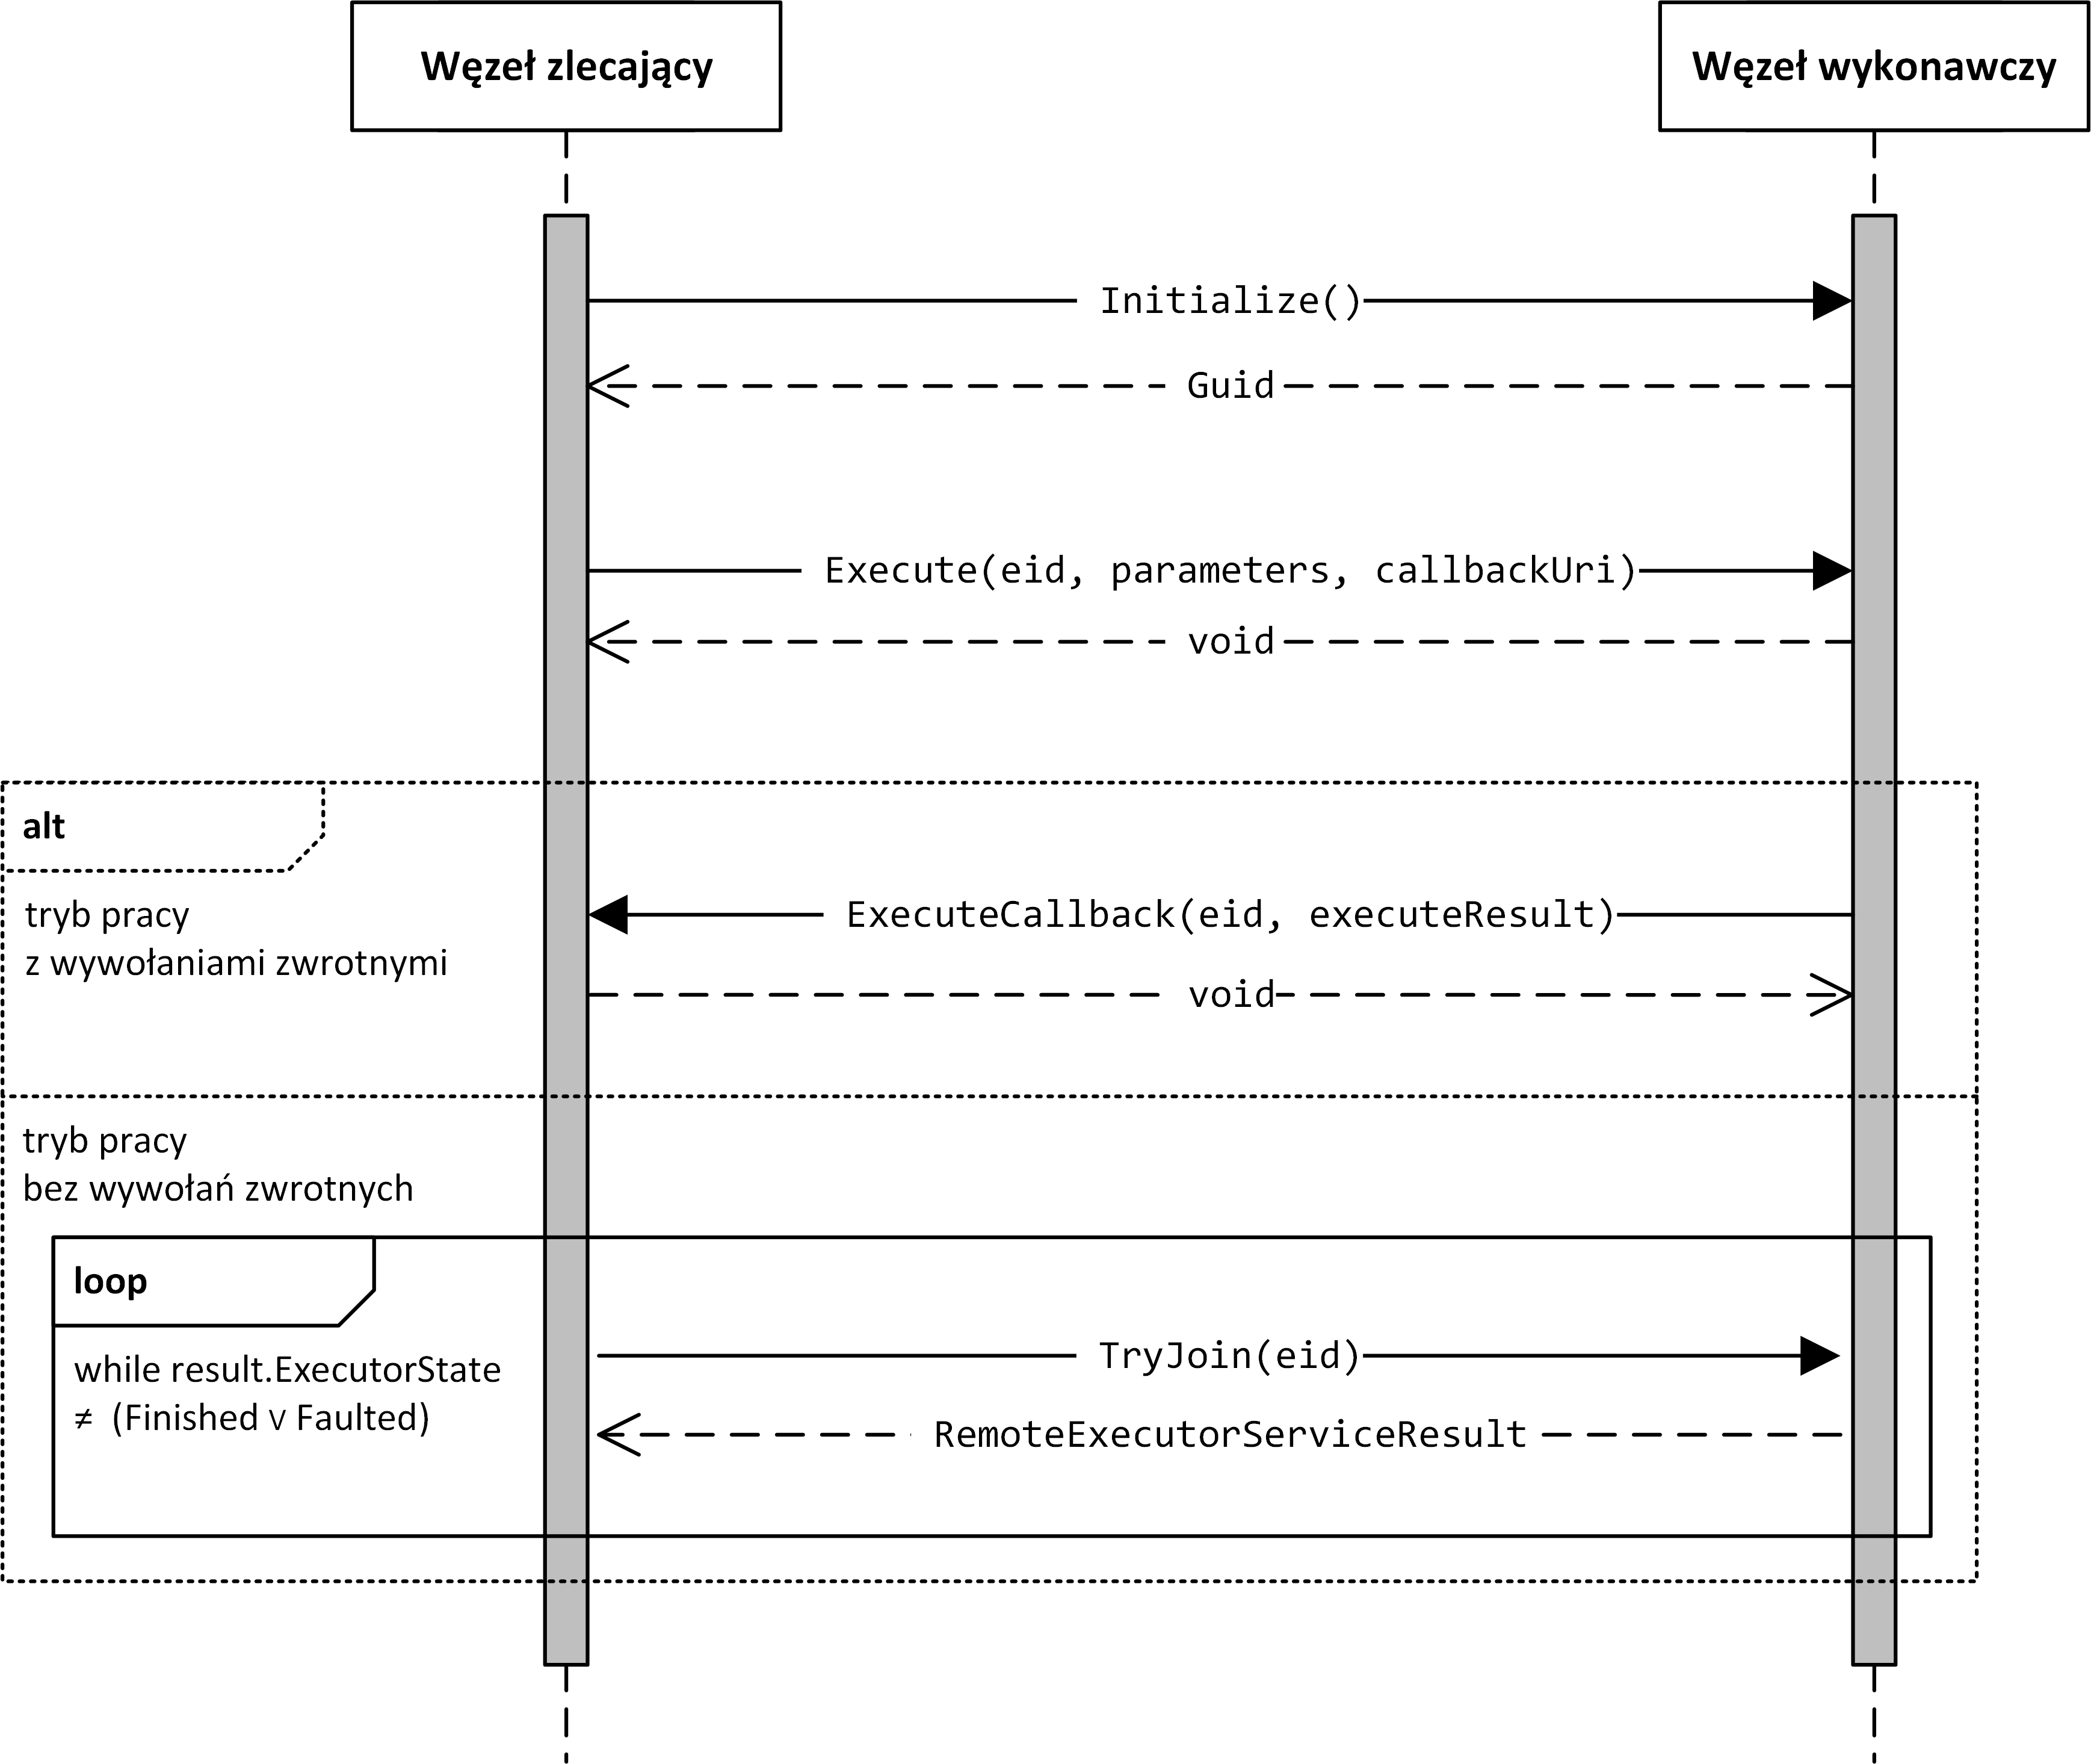
\includegraphics{images/diagram-protokolu}\protect\caption{\label{fig:implementation-Protokol-IRemoteExecutorService}Diagram
protokołu komunikacyjnego węzłów obliczeniowych}
\end{figure}



\subsection{Inicjalizacja}

Każdy wykonawca jest identyfikowany przez \dcscode{eid} (ang. \dcsemph{Executor ID})
-- unikalną 128-bitową liczbę (GUID, ang. \dcsemph{Globally Unique Identifier}),
przy czym instancja \dcsname{zdalnego wykonawcy} używa takiego samego
identyfikatora jak \dcsname{lokalny wykonawca}, który został zainicjowany
do wykonania kodu użytkownika. Wiadomość inicjująca wątek \dcscode{Initialize}
zawiera element \dcscode{methodHandle}, w którym przesyłany jest
zserializowany binarnie i zapisany w kodowaniu Base64 uchwyt do metody.
W odpowiedzi przesyłany jest identyfikator wykonawcy. Listing \ref{lis:implementation-SOAP-Initialize}
przedstawia w skróconej formie przykładową przechwyconą kopertę SOAP
z wiadomością \dcscode{Initialize}.

\inputencoding{latin2}\begin{lstlisting}[caption={Koperta SOAP -- inicjalizacja
zdalnego wykonawcy},label={lis:implementation-SOAP-Initialize},language=XML,numbers=left]
<s:Envelope xmlns:s="http://schemas.xmlsoap.org/soap/envelope/">
	<s:Body>
		<Initialize xmlns="http://tempuri.org/">
			<methodHandle>AAEAAAD/////AQAAAAAAAAAMAgAAAD9[...]==</methodHandle>
		</Initialize>
	</s:Body>
</s:Envelope>
\end{lstlisting}
\inputencoding{utf8}

Listing \ref{lis:implementation-SOAP-Initialize-decBase64} prezentuje
fragment uchwytu do metody po zdekodowaniu i usunięciu znaków spoza
drukowalnego zestawu symboli ASCII. DistributedPI to przykładowy program
opisany szerzej w punkcie \ref{sec:Przykladowe-zastosowania-liczba-pi}.
Uchwyt dotyczy metody anonimowej (stąd wygenerowana przez kompilator
nazwa \dcscode{b\_\_0}) zdefiniowanej w klasie \dcscode{Bluepath.DistributedPI.Program},
która jako parametr przyjmuje \dcscode{int} (\dcscode{System.Int32})
a typem zwracanym jest \dcscode{long} (\dcscode{System.Int64}). 

\inputencoding{latin2}\begin{lstlisting}[caption={Zdekodowany fragment
uchwytu do anonimowej metody},label={lis:implementation-SOAP-Initialize-decBase64},language=Assembler,numbers=left]
[...] System.Type[]
<RunTest>b__0 MBluepath.DistributedPI, Version=1.0.0.0, Culture=neutral, 
PublicKeyToken=null Bluepath.DistributedPI.Program
Int64 <RunTest>b__0(Int32) (System.Int64 <RunTest>b__0(System.Int32) 
System.UnitySerializationHolder Data	UnityType AssemblyName
\end{lstlisting}
\inputencoding{utf8}


\subsection{Przesłanie parametrów, wykonanie}

W kolejnej wiadomości, po inicjalizacji, węzeł zlecający przesyła
parametry wywołania metody. Przechwycona koperta z komunikatem \dcscode{Execute}
znajduje się na listingu \ref{lis:implementation-SOAP-Execute}. Warto
zauważyć, że ustawiona jest tutaj wartość pola \dcscode{callbackUri},
co~oznacza, że węzeł wywołujący otrzyma komunikat \dcscode{ExecuteCallback}
po zakończeniu przetwarzania po zdalnej stronie.

\inputencoding{latin2}\begin{lstlisting}[caption={Koperta SOAP -- przes�anie
paramter�w},label={lis:implementation-SOAP-Execute},breaklines=true,language=XML,numbers=left]
<s:Envelope xmlns:s="http://schemas.xmlsoap.org/soap/envelope/">
	<s:Body>
		<Execute xmlns="http://tempuri.org/">
			<eId>6a3ff0e2-601b-4683-a163-7f6da037c762</eId>
			<parameters xmlns:a="http://schemas.microsoft.com/2003/10/Serialization/Arrays" xmlns:i="http://www.w3.org/2001/XMLSchema-instance">
				<a:anyType i:type="b:int" xmlns:b="http://www.w3.org/2001/XMLSchema">10000</a:anyType>
			</parameters>
			<callbackUri xmlns:a="http://schemas.datacontract.org/2004/07/Bluepath.Services" xmlns:i="http://www.w3.org/2001/XMLSchema-instance">
				<a:Address>http://192.168.0.7:51000/BluepathExecutorService.svc</a:Address>
				<a:BindingType>BasicHttpBinding</a:BindingType>
			</callbackUri>
		</Execute>
	</s:Body>
</s:Envelope>
\end{lstlisting}
\inputencoding{utf8}

Lokalny wykonawca szereguje wątki do wykonania używając dostarczonej
przez środowisko .NET Framework puli wątków (\dcscode{ThreadPool}).
Podejście to ma swoje wady -- tracona jest kontrola nad tak stworzonymi
wątkami, nie można ich przerwać lub sprawdzić ich stanu (uniemożliwia
to np. realizację detekcji zakleszczenia). Biblioteka Bluepath zapewnia,
że w przypadku, gdy w kodzie użytkownika wystąpi wyjątek, zostanie
on przechwycony, zserializowany i udostępniony wywołującemu wątkowi
do odczytu.


\subsection{Wywołanie zwrotne}

Po zakończeniu metody w trybie z wywołaniem zwrotnym, zdalna strona
przesyła wynik, ew. wyjątki oraz czas jaki zajęło przetwarzanie do
zlecającej maszyny. Przykładowy komunikat \dcscode{ExecuteCallback}
przedstawia listing \ref{lis:implementation-SOAP-ExecuteCallback}.

\noindent %
\begin{minipage}[t]{1\textwidth}%
\inputencoding{latin2}\begin{lstlisting}[caption={Koperta SOAP -- wywo�anie
zwrotne z wynikiem},label={lis:implementation-SOAP-ExecuteCallback},breaklines=true,language=XML,numbers=left]
<s:Envelope xmlns:s="http://schemas.xmlsoap.org/soap/envelope/">
	<s:Body>
		<ExecuteCallback xmlns="http://tempuri.org/">
			<eid>6a3ff0e2-601b-4683-a163-7f6da037c762</eid>
			<executeResult xmlns:a="http://schemas.datacontract.org/2004/07/Bluepath.Services" xmlns:i="http://www.w3.org/2001/XMLSchema-instance">
				<a:ElapsedTime>PT0.0125743S</a:ElapsedTime>
				<a:Error i:nil="true" xmlns:b="http://schemas.datacontract.org/2004/07/System"/>
				<a:ExecutorState>Finished</a:ExecutorState>
				<a:Result i:type="b:long" xmlns:b="http://www.w3.org/2001/XMLSchema">7857</a:Result>
			</executeResult>
		</ExecuteCallback>
	</s:Body>
</s:Envelope>
\end{lstlisting}
\inputencoding{utf8}%
\end{minipage}


\section{Planista}

Wraz z systemem dostarczone zostały następujące typy \dcsname{planistów}: 
\begin{itemize}
\item \dcscode{ThreadNumberScheduler} -- szereguje zadania na najmniej
obciążonym węźle pod względem liczby wykonywanych na nim wątków,
\item \dcscode{RoundRobinScheduler} -- szereguje zadania korzystając z
algorytmu cyklicznego (ang.~\dcsemph{round robin}) \cite{Tannenbaum-SOP}.
\end{itemize}
Wszystkie implementacje \dcsname{planisty} muszą implementować interfejs
\dcscode{IScheduler} dzięki czemu można zastosować implementację
\dcsname{planisty} dostosowaną do potrzeb przetwarzania i jest jednym
z elementów modułowości systemu. Poniżej zostały szczegółowo opisane
implementacje planistów dostarczonych z systemem. 


\subsection{Szeregowanie zadań w oparciu o obciążenie węzłów}

\label{sub:implementacja-szeregowanie-zadan-threadcount}Jednym z
podstawowych sposobów szeregowania zadań jest próba równomiernego
rozłożenia obciążenia węzłów. Zakładając, że wszystkie zadania mają
podobny rozmiar, jako miarę obciążenia konkretnego węzła można przyjąć
liczbę zadań, które są obecnie przetwarzane, lub oczekują na rozpoczęcie
przetwarzania.

W przykładowej implementacji dostarczanej wraz z biblioteką \dcsname{Bluepath}
informacje o obecnym obciążeniu węzłów są okresowo odświerzane prz
pomocy \dcsname{usługi odnajdywania węzłów}. W zależności od
szybkości tworzenia nowych \dcsname{wątków rozproszonych} oraz
częstotliwości odświerzania informacji o obciążeniu węzłów lokalne
dane mogą szybko stać się nieaktualne. Można ten efekt złagodzić poprzez
zwiększanie zapamiętanego obciążenia o wysłane na dany węzeł wątki.


\subsection{Szeregowanie zadań za pomocą algorytmu cyklicznego}

\label{sub:Implementacja-Szeregowanie-karuzelowy}W pewnych zastosowaniach
pewne zrównowarzenie obciążenia można osiągnąć poprzez zastosowanie
algorytmu cyklicznego. Algorytm ten nie wymaga pobierania informacji
o obciążeniu węzłów z \dcsname{usługi odnajdywania węzłów}, przez
co posiada mniejszy narzut komunikacyjny od algorytmów wymagających
tych informacji. 


\section{Pamięć rozproszona}

Ponieważ celem pracy nie było kompletne implementowanie pamięci rozproszonej,
skupiono się na wyborze istniejącego rozwiązania, które spełniałoby
wymagania zaprezentowane w punkcie \ref{sec:concept-Rozproszona-pami=000119=000107-wsp=0000F3=000142dzielona}.


\subsection{Rozważane rozwiązania }

\label{sub:implementation-Pamiec-rozproszona-rozwazane-rozwiazania}Początkowo
pod uwagę brane były następujące aplikacje:
\begin{itemize}
\item Memcached \cite{Memcached} -- system dostarczający rozproszoną pamięć
przechowującą dane w postaci par klucz-wartość. Nie znaleziono aktywnie
rozwijanego klienta dla platformy .NET,
\item Riak \cite{Riak} -- implementacja Amazon Dynamo \cite{Amazon-Dynamo},
odrzucony ze względu na brak API dla .NET Framework,
\item Polyphony \cite{Polyphony-blog-1,Polyphony-blog-2,Polyphony-blog-3,Polyphony-repo}
-- eksperymentalny projekt rozproszonej tablicy haszowej napisany
w języku F\#, nie wybrano ze względu na wczesnorozwojowy charakter
projektu,
\item Rhino DHT \cite{Rhino-DHT} -- implementacja rozproszonej tablicy
haszowej w języku C\#; posiada zależności od Rhino PHT (\dcsemph{persistent hash table})
\cite{Rhino-PHT} oraz Rhino Queues \cite{Rhino-Queues},
\end{itemize}
a w późniejszym okresie również:
\begin{itemize}
\item Redis \cite{Redis} -- system rozpowszechniany na licencji \dcsemph{open source}
przechowujący dane typu klucz-wartość.
\end{itemize}
Pierwszym wybranym rozwiązaniem było Rhino DHT, które było aktywnie
rozwijane przez rozpoznawalnego autora -- Ayende Rahiena. Niestety,
okazało się, że wersjonowanie danych nie zostało w pełni zaimplementowane
i nie było możliwe wykonanie atomowej operacji ,,odczytaj i zapisz'',
która była niezbędna do zrealizowania \dcsname{zamków rozproszonych}.
Szczegóły tego problemu zostały przedstawione w~punkcie \ref{par:problemy-rhino-dht}. 

Kolejnym rozwiązaniem wziętym pod uwagę był Redis -- system autorstwa
Salvatore Sanfilippo oraz Pietera Noordhuisa. Jest używany na co dzień
jako mechanizm pamięci podręcznej wielu serwisów internetowych (m.~in.
cała rodzina StackExchange) -- posiada przez to duże wsparcie i aktywnie
działającą społeczność. Redis potrafi działać zarówno jako pojedynczy
proces jak i w trybie master-slave, ponadto rozwijana jest wersja
rozproszona -- Redis Cluster. System ten posiada biblitekę dla .NET
Framework dostarczoną przez firmę StackExchange. Redis został napisany
dla rodziny systemów operacyjnych Linux, powstał jednak port tego
systemu do systemu operacyjnego Windows. Problemy, które napotkano
podczas uruchamiania usługi Redis (opisane w punkcie \ref{par:problemy-Windows-Redis})
udało się rozwiązać, przez co system ten został wykorzystany w ostatecznej
wersji pracy i w testach.


\subsection{Interfejsy pamięci rozproszonej}

Definicje \dcsname{pamięci rozproszonej} oraz \dcsname{rozszerzonej pamięci rozproszonej}
zostały sformalizowane w formie interfejsów odpowiednio \dcscode{IStorage}
oraz \dcscode{IExtendedStorage}. Interfejs \dcscode{IStorage} wymaga
implementacji metod do operacji na pojedynczych wartościach: \dcscode{Store},
\dcscode{StoreOrUpdate}, \dcscode{Update}, \dcscode{Retrieve} i
\dcscode{Remove} oraz operacji zbiorczych: \dcscode{BulkStore},
\dcscode{BulkStoreOrUpdate}, \dcscode{BulkUpdate}, \dcscode{BulkRetrieve}
i \dcscode{BulkRemove}. Semantyka tych operacji odpowiada operacjom
zdefiniowanym w punkcie \ref{sec:concept-Rozproszona-pami=000119=000107-wsp=0000F3=000142dzielona}.
Wszystkie operacje zdefiniowane w \dcsname{pamięci rozproszonej}
i \dcsname{rozszerzonej pamięci rozproszonej} pozwalają na bezpieczne
współbieżne wywołanie z wielu wątków (ang. \dcsemph{thread-safe}). 

Interfejs \dcscode{IExtendedStorage} rozszerza podstawowy interfejs
\dcscode{IStorage} o operacje pobrania i zwolnienia \dcsname{zamków rozproszonych}:
\dcscode{AcquireLock} (w wersji z limitem czasu oczekiwania na pobranie
zamka i bez) oraz \dcscode{ReleaseLock}. 


\subsection{Rozproszone struktury danych i obiekty}

Struktury danych i obiekty, które mogą być współdzielone między \dcsname{wątkami rozproszonymi}
zaimplementowane zostały w oparciu o \dcsname{pamięć rozproszoną},
zdefiniowaną za pomocą interfejsu \dcscode{IExtendedStorage} -- pozwoliło
to zastosować \dcsname{zamki rozproszone} w celu zapewnienia poprawności
przetwarzania -- współbieżny dostęp do rozproszonych struktur danych
i obiektów może być prowadzony zarówno z wątków jak i \dcsname{wątków rozproszonych}.
Każdy obiekt jest identyfikowany przez klucz będący łańcuchem znaków.
W przypadku listy czy słownika na podstawie klucza wywiedzione zostają
identyfikatory obiektów składających się na daną strukturę -- zamków,
metadanych i poszczególnych wartości. 


\subsubsection*{Lista}

Lista implementuje standardowy generyczny interfejs \dcscode{IList<T>}
z przestrzeni nazw \dcscode{System.Collections.Generic}. Próba pobrania
enumeratora zwraca obiekt klasy \dcscode{DistributedListEnumerator},
który umożliwia iterowanie po kolekcji. \dcsname{Lista rozproszona}
została rozszerzona o operację \dcscode{CopyPartTo} -- jest to odpowiednik
operacji \dcscode{CopyTo} (efektywnej operacji kopiowania całej zawartości
listy do wskazanej tablicy), który pozwala skopiować wybrany fragment
listy w sposób efektywny i atomowy. Operacja ta jest szczególnie przydatna
przy przetwarzaniu rozproszonym, gdzie dane znajdują się w wolnej
\dcsname{pamięci rozproszonej} (w stosunku do pamięci podręcznej),
a~każdy \dcsname{wątek rozproszony} przetwarza fragment danych.


\subsubsection*{Słownik}

Słownik implementuje standardowy generyczny interfejs \dcscode{IDictionary<TKey, TValue>}
z przestrzeni nazw \dcscode{System.Collections.Generic}. Próba pobrania
enumeratora zwraca obiekt klasy \dcscode{DistributedDictionaryEnumerator},
który umożliwia iterowanie po kolekcji. 


\subsubsection*{Licznik}

W wielu scenariuszach (przykładowy scenariusz opisany w \ref{par:koncepcja-distributed-counter})
przydatnym obiektem może być \dcsname{licznik rozproszony}. Zaimplementowana
klasa \dcscode{DistributedCounter} udostępnia następujące operacje: 
\begin{itemize}
\item \dcscode{GetValue} -- pobiera aktualną wartość licznika,
\item \dcscode{SetValue} -- ustawia podaną liczbę jako wartość licznika,
\item \dcscode{Increase} -- zwiększa wartość licznika o podaną wartość,
\item \dcscode{Decrease} -- zmniejsza wartość licznika o podaną wartość,
\item \dcscode{GetAndIncrease} -- atomowo pobiera aktualną wartość licznika
i zwiększa ją o~wskazaną liczbę, gdzie liczba o którą ma zostać zwiększony
licznik może być ujemna.
\end{itemize}

\subsection{Zamki rozproszone}

Odpowiednikiem definicji \dcsname{zamków rozproszonych} z punktu
\ref{sub:Koncepcja-Zamki-rozproszone} jest interfejs \dcscode{IStorageLock}.
Zdefiniowane w nim zostały następujące operacje:
\begin{itemize}
\item \dcscode{Acquire} -- operacja pobrania zamka. Posiada wariant, który
pozwala określić czas oczekiwania na pobranie zamka -- jeśli czas
ten zostanie przekroczony przed pobraniem zamka użytkownik dostanie
informację o niepowodzeniu i~będzie mógł kontynuować przetwarzanie.
Operacja pobrania zamka bez podania czasu oczekiwania jest blokująca
-- przetwarzanie będzie kontynuowane dopiero po pobraniu zamka,
\item \dcscode{Release} -- operacja zwolnienia zamka,
\item \dcscode{Wait} -- wykonanie tej operacji powoduje rozpoczęcie oczekiwania
na sygnał (ang.~\dcsemph{pulse}) od innego procesu. Wykonanie tej
operacji powoduje tymczasowe zwolnienie dostępu do zamka. Po otrzymaniu
sygnału proces próbuje ponownie pobrać zamek. Podobnie jak \dcscode{Acquire}
operacja ta posiada wariant, który pozwala określić czas oczekiwania
na sygnał,
\item \dcscode{Pulse} i \dcscode{PulseAll} -- wykonanie tych operacji
powoduje wysłanie sygnału do procesów oczekujących na operacji \dcscode{Wait}.
W pierwszym przypadku sygnał dotrze do conajmniej jednego oczekującego
procesu, a w drugim do wszystkich oczekujących procesów.
\end{itemize}
Interfejs \dcscode{IStorageLock} dziedziczy z interfejsu \dcscode{IDisposable}
-- sprawia to, że zamek można wykorzystać w podobny sposób jak słowo
kluczowe \dcscode{lock}, korzystając w tym celu z bloku \dcscode{using},
co przedstawiono na listingu \ref{lis:implementation-Realizacja-sekcji-krytycznej}.
Cechą bloku \dcscode{using} jest automatyczne wywołanie na jego końcu
operacji \dcscode{Dispose}, która w przypadku \dcsname{zamków rozproszonych}
powoduje zwolnienie zamka.

\noindent %
\begin{minipage}[t]{1\textwidth}%
\inputencoding{latin2}\begin{lstlisting}[caption={Realizacja
sekcji krytycznej z wykorzystaniem zamka rozproszonego},label={lis:implementation-Realizacja-sekcji-krytycznej},breaklines=true,language=bash,numbers=left]
using(var @lock = storage.AcquireLock("sampleLock"))
{
	// sekcja krytyczna
}
\end{lstlisting}
\inputencoding{utf8}%
\end{minipage}


\section{Logowanie zdarzeń}

\label{sec:implementation-Logowanie-zdarzen}Za zbieranie informacji
na temat zdarzeń zachodzących w systemie odpowiada klasa \dcscode{Log}
udostępniająca m. in. statyczne metody:
\begin{itemize}
\item \dcscode{ExceptionMessage} -- do logowania wyjątków,
\item \dcscode{TraceMessage} -- do logowania pozostałych zdarzeń.
\end{itemize}
Istnieje możliwość przekierowania wszystkich informacji do \dcsname{pamięci rozproszonej}.
W~tym celu należy ustawić flagę \dcscode{WriteToDistributedMemory}
oraz uzupełnić nazwę hosta \dcsname{pamięci rozproszonej} (\dcscode{DistributedMemoryHost}),
do którego ma odbywać się zapis. Warto zwrócić uwagę, że tryb pracy
ze zbieraniem historii zdarzeń w \dcsname{pamięci współdzielonej}
może istotnie ograniczać wydajność systemu. W celu zmaterializowania
zebranego logu udostępniona została metoda \dcscode{SaveXes}, która
zapisuje wszystkie zgromadzone w \dcsname{pamięci rozproszonej}
zdarzenia do pliku XML w formacie OpenXES. 

Implementacja zapisu zdarzeń do pliku XML została wykonana na podstawie
zmodyfikowanych plików XSD (pkt. \ref{def:background-XSD}) udostępnionych
wraz z biblioteką OpenXES \cite{OpenXES} w wersji 2.0 (przyczyny
i sposób modyfikacji został opisany w punkcie \ref{sub:problemy-Implementacja-standardu-OpenXES-z-XSD}).
Szkielet klas został wygenerowany przy użyciu narzędzia XML Schema
Definition Tool \cite{XML-Schema-Definition-Tool} (\dcscode{xsd.exe})
dostarczanego wraz ze środowiskiem programistycznym .NET Framework
4.5.1. Przykład użycia programu \dcscode{xsd.exe} został zaprezentowany
na listingu \ref{lis:implementation-Skrypt-generuj=000105cy-klasy-z-XSD}. 

\noindent %
\begin{minipage}[t]{1\textwidth}%
\inputencoding{latin2}\begin{lstlisting}[caption={Skrypt
generuj�cy klasy w j�zyku C\# na podstawie pliku XSD dla formatu OpenXES },label={lis:implementation-Skrypt-generuj=000105cy-klasy-z-XSD},breaklines=true,language=bash,numbers=left]
"c:\Program Files (x86)\Microsoft SDKs\Windows\v8.1A\bin\NETFX 4.5.1 Tools\xsd.exe" xes.xsd /classes /o:../Bluepath/Reporting/ 
"c:\Program Files (x86)\Microsoft SDKs\Windows\v8.1A\bin\NETFX 4.5.1 Tools\xsd.exe" xesext.xsd /classes /o:../Bluepath/Reporting/
\end{lstlisting}
\inputencoding{utf8}%
\end{minipage}

Wszystkie zdarzenia zachodzące w systemie zostały pogrupowane w tkw.
\dcsname{aktywności} (ang.~\dcsemph{activity}). Rodzaje aktywności
zachodzących w systemie zostały zdefiniowane w formie typu wyliczeniowego
\dcscode{Bluepath.Reporting.Log.Activity}, obejmuje on m. in.:
\begin{itemize}
\item \dcscode{Service\_is\_ready} -- zgłoszenie przez węzeł gotowości
do przyjęcia zleceń,
\item \dcscode{Local\_executor\_started\_running\_user\_code} -- rozpoczęcie
wykonywania kodu użytkownika w ramach rozproszonego wątku,
\item \dcscode{Local\_executor\_finished\_running\_user\_code} -- zakończenie
wykonywania kodu użytkownika na węźle,
\item \dcscode{Sending\_callback\_with\_result} -- wysłanie wywołania zwrotnego
z wynikiem działania wątku.
\end{itemize}
Wszystkie zdarzenia, które są mało istotne dla analizy procesu mogą
być grupowane w ramach aktywności \dcscode{Info} i powinny zostać
odfiltrowane w pierwszej fazie analizy. Jeżeli użytkownik chce użyć
własnej nazwy dla zdarzenia, może to zrobić korzystając z aktywności
\dcscode{Custom}, a właściwą nazwę przekazać jako parametr \dcscode{message}
do metody logowania zdarzeń. 

Format XES definiuje dla zdarzeń w logu \dcsname{zasób} (ang.~\dcsemph{resource})
-- w przypadku biblioteki \dcsname{Bluepath} wartością tego pola
jest zawsze wykonawca, który dokonał wpisu, korzystając z jego unikalnego
identyfikatora \dcscode{eid}. Implementacja zakłada możliwość skrócenia
zapisu do n ostatnich znaków składających się na identyfikator w celu
ułatwienia analizy przez człowieka. Może to potencjalnie wpłynąć na
fałszywe sklasyfikowanie różnych zasobów jako tego samego w wyniku
kolizji tak skonstruowanych identyfikatorów.

Zależności czasowe są istotną częścią analizy przebiegu procesu. Z
wykorzystaniem serwerów czasu implementujących protokół NTP (ang.
\dcsemph{network time protocol}) \cite{rfc5905} możliwe jest zsynchronizowanie
zegarów węzłów w klastrze z dokładnością do milisekund (przy dużych
odległościach od serwera czasu -- dziesiątek milisekund) \cite{Mills-NTP-IEEE-Trans}.
Może to być niewystarczające do jednoznacznego określenia porządku
zdarzeń. Klasa \dcscode{Log} zawiera flagę \dcscode{monotonicallyIncreasingLogTime},
której ustawienie uniemożliwia zapisanie dwóch zdarzeń z tym samym
znacznikiem czasowym poprzez realizowanie dodatkowych operacji podczas
zapisu do logu:
\begin{itemize}
\item pobranie \dcsname{zamka rozproszonego},
\item odczyt ostatnio zapisanej wartości znacznika czasowego z \dcsname{pamięci rozproszonej},
\item w przypadku gdy lokalna wartość znacznika jest mniejsza lub równa
odczytanemu, jest ona zamieniana na odczytaną wartość zwiększoną o
1 milisekundę,
\item zapis bieżącej wartości znacznika czasowego do \dcsname{pamięci rozproszonej},
\item zwolnienie \dcsname{zamka rozproszonego}.
\end{itemize}



\section{Interfejs do komunikacji z systemem}

Aby skorzystać z funkcji udostępnianych przez system (jak np. pobranie
identyfikatora \dcsname{wykonawcy} czy dostęp do \dcsname{pamięci rozproszonej})
wewnątrz \dcsname{wątku rozproszonego}, użytkownik musi uzyskać
przeznaczony do tego obiekt. System automatycznie wstrzykuje go do
metod jako jeden z parametrów -- wystarczy, by był on typu \dcscode{IBluepathCommunicationFramework}.
Użytkownika ma również możliwość zapisywania własnych zdarzeń zachodzących
w aplikacji do logu z użyciem opisanej w punkcie \ref{sec:implementation-Logowanie-zdarzen}
statycznej klasy \dcscode{Log}.


\section{Dystrybucja aplikacji w klastrze}

\label{sec:implementation-Skrypt-Send-Folder}PowerShell Remoting
\cite{PS-Remoting} to usługa umożliwiająca wykonanie na zdalnych
maszynach pojedynczych komend lub stworzenie pełnej zdalnej sesji
PowerShell. Automatyzacja procesu dystrybucji plików binarnych systemu
w klastrze została zrealizowana za pomocą zestawu skryptów: \dcspath{Send-Folder}
do przesyłania całych folderów i \dcspath{Send-File} do przesyłania
pojedynczych plików, z którego korzysta ten pierwszy. 

Skrypt do wysyłania pojedynczych plików został zaczerpnięty z książki
\cite{Windows-PowerShell-Cookbook}. Przyjmuje 3 parametry: ścieżkę
do pliku źródłowy znajdującego się na lokalnej maszynie, ścieżkę docelową
na zdalnej maszynie oraz referencję do obiektu zdalnej sesji. Plik
jest wczytywany do pamięci jako tablica bajtów, następnie jego transfer
odbywa się strumieniowo w blokach o rozmiarze 1 MB. Po zrekonstruowaniu
tablicy bajtów na zdalnej stronie jest ona zapisywana na dysk we wskazanej
lokalizacji.

Skrypt do wysyłania folderów przedstawiony na listingu \ref{lis:implementation-Send-Folder}
przyjmuje jako parametry: 
\begin{itemize}
\item adres zdalnego komputera (\dcscode{-server}), 
\item opcjonalnie port, na którym nasłuchuje usługa PowerShell Remoting
(\dcscode{-port}), 
\item nazwę użytkownika (\dcscode{-user}), 
\item hasło (\dcscode{-password}), 
\item ścieżkę do folderu źródłowego na lokalnej maszynie (\dcscode{-source}), 
\item oraz ścieżkę do folderu docelowego na zdalnej maszynie (\dcscode{-destination}). 
\end{itemize}
Skrypt tworzy obiekt zdalnej sesji uwierzytelniając się poprzez podaną
nazwę użytkownika i hasło. W celu uproszczenia etapu konfiguracji
środowiska, do wywołania metody \dcscode{New-PSSession} można dodać
przełącznik \dcscode{-SessionOption} z parametrem \dcscode{New-PSSessionOption -SkipCACheck}.
Opcja ta powoduje jednak obniżenie poziomu bezpieczeństwa poprzez
dopuszczenie niezaufanych certyfikatów maszyn. Następnie pobierana
jest lista plików we wskazanym lokalnym folderze i dla każdego z plików
wywoływany skrypt \dcspath{Send-File}. Pomijane przy tym są pliki
z symbolami (\dcspath{.pdb}), ponieważ ich rozmiar jest znaczący
w stosunku do rozmiaru plików samej aplikacji, a nie było konieczne
podłączanie \dcsemph{debuggera} do procesów pracujących na zdalnych
maszynach. Po zakończeniu przesyłania plików zdalna sesja jest zamykana.
Warto zauważyć, że skrypt \dcspath{Send-Folder} można wywołać wielokrotnie
przekazując w parametrze -server kolejne adresy maszyn, aby rozdystrybuować
pliki w całym klastrze.

\inputencoding{latin2}\begin{lstlisting}[caption={Skrypt przesy�aj�cy pliki ze
wskazanego folderu na zdaln� maszyn�},label={lis:implementation-Send-Folder},language=bash,numbers=left]
param (
	[string]$server = $(throw "-server is required."),
	[int]$port = 5986,
	[string]$user = $(throw "-user is required."),
	[string]$password = $(throw "-password is required."),
	[string]$source = $(throw "-source is required."),
	[string]$destination = $(throw "-destination is required.")
)

$secPassword = ConvertTo-SecureString $password -AsPlainText -Force
$credential = New-Object System.Management.Automation.PSCredential($user, $secPassword)
$uri = New-Object System.Uri("https://" + $server + ":" + $port)

$session = New-PSSession -ConnectionUri $uri -Credential $credential

Get-ChildItem -Path $source -File | Foreach-Object {
	if ($_.Extension -ne ".pdb") {
		$target = $destination + $_.Name
		.\Send-File.ps1 $_.FullName $target $session
	}
}

Disconnect-PSSession $session
\end{lstlisting}
\inputencoding{utf8}
